\documentstyle[11pt,epsfig,fancybox,semcolor,semlayer,doublespace,portrait]
{seminar}
\input clp_utils

\def\cesr{{\sc Cesr}}
\def\cleo{{\sc Cleo}}
\def\cleoii{{\sc Cleo II}}
\def\cleoiii{{\sc Cleo III}}
\def\cleoc{{\sc Cleo}-c}
\def\lepp{{\sc Lepp}}

% The following strings are needed by the title page and 
% page style definitions in map_utils.tex
\newcommand{\talktitle}[0]{ }
\newcommand{\fmttitle}[0]{}
\newcommand{\conftitle}[0]{ }
\newcommand{\myname}[0]{Jim Pivarski}
\newcommand{\affila}[0]{ }
\newcommand{\talkdate}[0]{April 3, 2003}

\pagestyle{conference}   % From clp_utils.tex

% slide magnification
\slidesmag 1

%%%%%%%%%%%%%%%%%%%%%%%%%%%%%%%%%%%%%%%%%%%%%%%%%%%%%%%%%%%%%%%%%%%%%%%%%%%
% Start document
\begin{document}

% Set page size
\slideheight 7.0in
\slidewidth 8.8in 

% Set array stretch
\renewcommand{\arraystretch}{0.3}
\renewcommand{\slidetopmargin}{0.4in}
\renewcommand{\slidebottommargin}{0.9in}

% %%%%%%%%%%%%%%%%%%%%%%%%%%%%%%%%%%%%%%%%%%%%%%%%%%%%%%%%%%%%%%%%%%%%%%%%%%%

\begin{slide*}
\slideframe{}
\slideframe*[\dkblue]{Oval}
\begin{minipage}[t]{\linewidth}
\Large \black

\begin{center}
  \begin{tabular}{l r}
    \begin{minipage}{0.1\linewidth}
      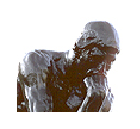
\epsfig{file=think.eps, width=\linewidth}
    \end{minipage} &
    \begin{minipage}{0.8\linewidth}

      \cleo's a dead end.  If you join the collaboration now, they'll
      just be shutting down in a few months\ldots

    \end{minipage} \\
    & \vspace{1cm} \\
    \begin{minipage}{0.1\linewidth}
      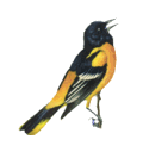
\epsfig{file=squawk.eps, width=\linewidth}
    \end{minipage} &
    \begin{minipage}{0.8\linewidth}

      No!  \cleoc\ will be running until 2006, and the analysis will
      keep going for years after that (many years).  You won't be a
      gradutate student long enough for {\it that} to matter.

    \end{minipage} \\
  \end{tabular}
  \vspace{2cm} \\
  \epsfig{file=timeline.eps, width=\linewidth}
\end{center}

\vspace{1.5cm}

Analysis continues long after data-taking is finished.  Most current
\cleo\ graduate students are analyzing data that finished running in
1999.

\end{minipage}
\end{slide*}

% %%%%%%%%%%%%%%%%%%%%%%%%%%%%%%%%%%%%%%%%%%%%%%%%%%%%%%%%%%%%%%%%%%%%%%%%%%%

\begin{slide*}
\slideframe{}
\slideframe*[\dkblue]{Oval}
\begin{minipage}[t]{\linewidth}
\huge \black

\begin{center}
  \begin{tabular}{l r}
    \begin{minipage}{0.1\linewidth}
      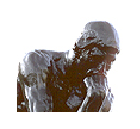
\epsfig{file=think.eps, width=\linewidth}
    \end{minipage} &
    \begin{minipage}{0.8\linewidth}

      If you're interested in software, they'll have you writing
      C-to-Fortran interfaces for the rest of your life\ldots

    \end{minipage} \\
    & \vspace{2cm} \\
    \begin{minipage}{0.1\linewidth}
      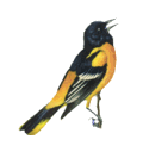
\epsfig{file=squawk.eps, width=\linewidth}
    \end{minipage} &
    \begin{minipage}{0.8\linewidth}

      {\Huge \sc \bf No!} {\LARGE (Unless you like C-to-Fortran interfaces.)} \\

    \end{minipage} \\
  \end{tabular}
  \vspace{2cm} \\
\end{center}

At \cleo, we do experiments {\it using} computers in much the
same way as one might experiment {\it using} an oscilloscope.

\vspace{1cm}

In this talk, I'll tell you about my experiences \mbox{experimenting} {\it
through} a computer.

\end{minipage}
\end{slide*}

% %%%%%%%%%%%%%%%%%%%%%%%%%%%%%%%%%%%%%%%%%%%%%%%%%%%%%%%%%%%%%%%%%%%%%%%%%%%

\begin{slide*}
\slideframe{}
\slideframe*[\dkblue]{Oval}
\begin{minipage}[t]{\linewidth}
\Large \black

{\huge Calibration Project: Detector Alignment}

\begin{quote}
  After the detectors have been moved into position to mm accuracy, we
  need to know {\emph where} they are to $\mu$m accuracy to precisely
  reconstruct a track.
\end{quote}

This is a plot I made to demonstrate a Toy Monte Carlo to investigate
stretching and squishing of the central drift chamber, and its effect
on track reconstruction.

%% (You're looking at an $e^+ e^- \to e^+ e^-$ event in the XY plane.
%% Blue tracks are reality, red are misreconstruction due to
%% unaccounted-for distortions in detector shape.)

%% \begin{itemize}
%%   \normalsize

%%   \item The physics event of choice is $e^+ e^- \to e^+ e^-$ where you
%%   get two back-to-back tracks, coming from the origin (blue).  This is
%%   an XY-projection.  The tracks are slightly curved because of the
%%   magnetic field.

%%   \item The 31-layer detector is modelled here with three
%%   representative layers.  The track-layer intersections (blue) are
%%   where the measurements took place in real space.

%%   \item The dashed layers and red points represent unaccounted-for
%%   distortions in the detector shape.

%%   \item I did an incorrect fit to the incorrect points (red lines) to
%%   see what effect these distortions would have on
%%   na\"ievely-reconstructed tracks.

%% \end{itemize}

\begin{center}
  \epsfig{file=way_misaligned.eps, height=\linewidth, angle=-90}
\end{center}

\end{minipage}
\end{slide*}

% %%%%%%%%%%%%%%%%%%%%%%%%%%%%%%%%%%%%%%%%%%%%%%%%%%%%%%%%%%%%%%%%%%%%%%%%%%%

\begin{slide*}
\slideframe{}
\slideframe*[\dkblue]{Oval}
\begin{minipage}[t]{\linewidth}
\Large \black

{\huge A Simple Example: Impact Parameter ($d$) versus $\phi$}

\vspace{0.25cm}

\begin{center}
  \begin{tabular}{l r}
    \begin{minipage}{0.2\linewidth}
      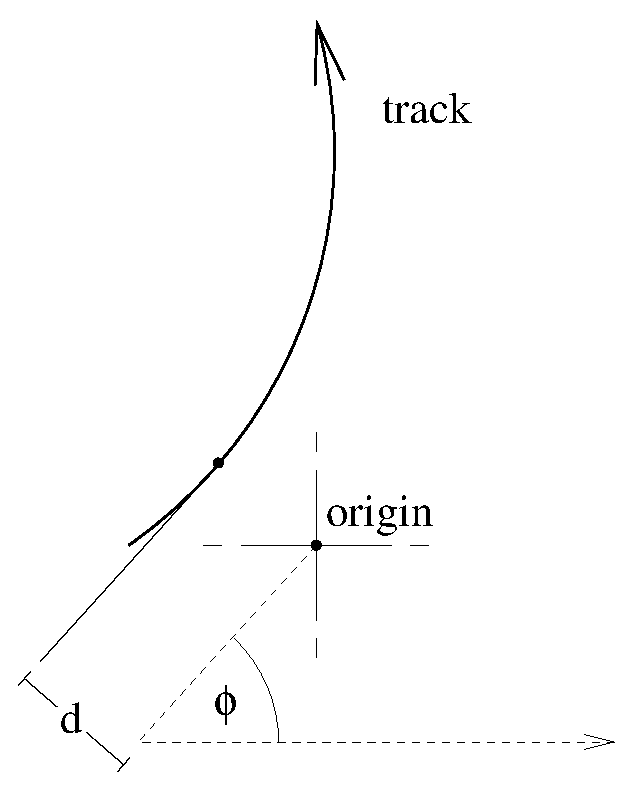
\epsfig{file=definitions.eps, width=\linewidth}
    \end{minipage} &
   \begin{minipage}{0.6\linewidth}
%     \setlength{\baselineskip}{1.5\baselineskip}
     \begin{itemize}

       \item $d$ is the closest a track gets to \mbox{the origin} (in the XY plane)

	\vspace{0.25cm} 

       \item $\phi$ is the direction of the track at that point

     \end{itemize}
   \end{minipage}
  \end{tabular}
  \vspace{0.5cm}
\end{center}

Most tracks should come from the origin (the collision point), so they
should be distributed around $d$ = 0.

\vspace{0.25cm}

\begin{center}
  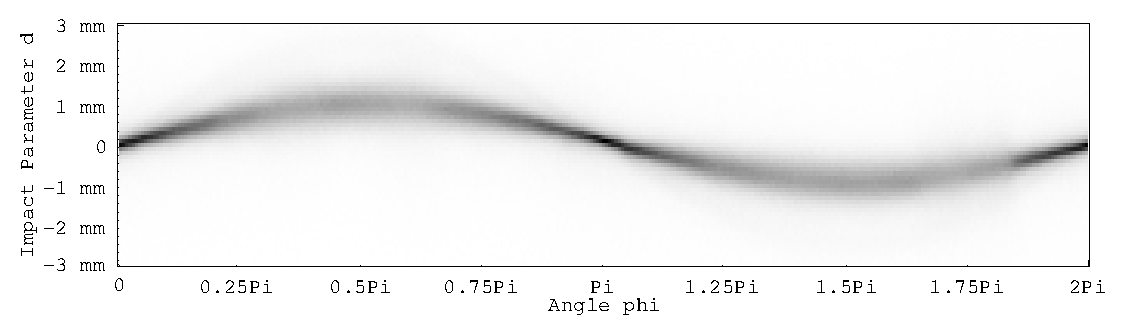
\epsfig{file=unshifted.eps, width=0.9\linewidth}
\end{center}

$\Longrightarrow$ tracks are actually originating at $x = -1$ mm:
\begin{center}
  \epsfig{file=cycled0.eps, width=0.75\linewidth}
\end{center}

Adjust origin:
\begin{center}
  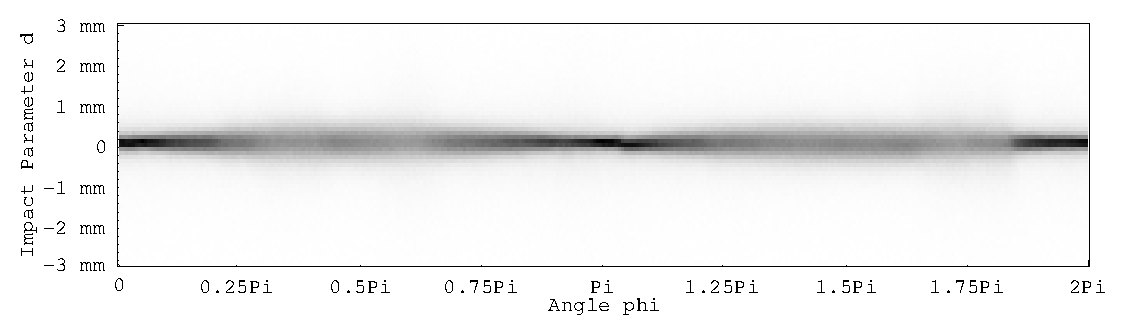
\epsfig{file=shifted.eps, width=0.9\linewidth}
\end{center}

\end{minipage}
\end{slide*}

% %%%%%%%%%%%%%%%%%%%%%%%%%%%%%%%%%%%%%%%%%%%%%%%%%%%%%%%%%%%%%%%%%%%%%%%%%%%

\begin{slide*}
\slideframe{}
\slideframe*[\dkblue]{Oval}
\begin{minipage}[t]{\linewidth}

\begin{center}
  \epsfig{file=hand_alignment.eps, width=0.95\linewidth, angle=180}
\end{center}

\end{minipage}
\end{slide*}

%%%%%%%%%%%%%%%%%%%%%%%%%%%%%%%%%%%%%%%%%%%%%%%%%%%%%%%%%%%%%%%%%%%%%%%%%%%

\begin{slide*}
\slideframe{}
\slideframe*[\dkblue]{Oval}
\begin{minipage}[t]{\linewidth}

\begin{center}
  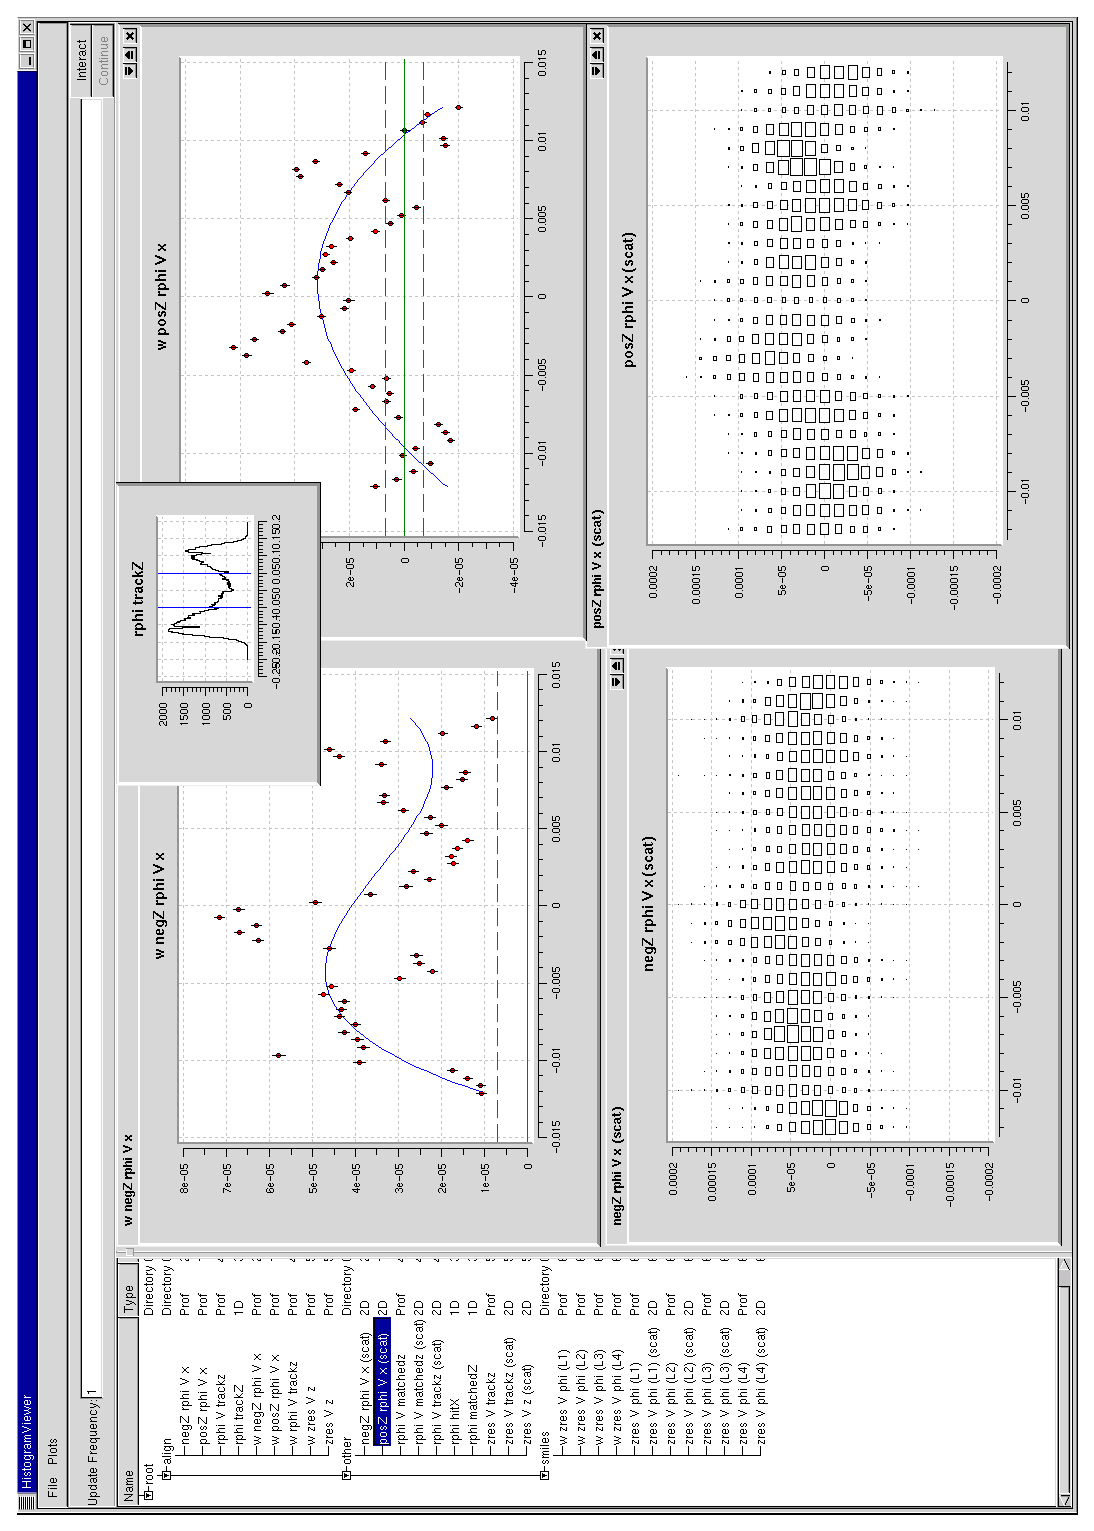
\epsfig{file=structure_found.eps, width=0.85\linewidth, angle=180}
\end{center}

\end{minipage}
\end{slide*}

%% % %%%%%%%%%%%%%%%%%%%%%%%%%%%%%%%%%%%%%%%%%%%%%%%%%%%%%%%%%%%%%%%%%%%%%%%%%%%

\begin{slide*}
\slideframe{}
\slideframe*[\dkblue]{Oval}
\begin{minipage}[t]{\linewidth}
\Large \black

{\huge Thesis project: measure yield of $e^+ e^- \to \Upsilon$} \\
\mbox{\hspace{4.5cm} ($b$-quark, $\bar{b}$-quark bound state)}

\vspace{1cm}

The beam energy of $e^+ e^-$ was set to the mass of the $\Upsilon$
bound state, and we measure the cross-section $e^+ e^- \to \Upsilon$.
The beam energy was varied to map out the lineshape of the resonance.
The yield is

\vspace{0.5cm}

\[ \int d\mbox{\sc Energy} \ \sigma(e^+ e^- \to \Upsilon) =
   \int d\mbox{\sc Energy} \ \frac{\sigma(e^+ e^- \to \Upsilon \to \mbox{hadrons})}
        {{\mathcal B}(\Upsilon \to \mbox{hadrons})} \]

%% Interfering effects:
%% \begin{itemize}

%%   \item Breit-Wigner (Lorentzian) lineshape is convoluted with a
%%   spread in beam energies that is an order of magnitude wider.  (Good
%%   thing I'm only interested in the area!)

%%   \item Beam electrons can radiate a photon before interacting
%%     (calculable QED process), gives the lineshape a high-energy tail.

%%   \item I measure $e^+ e^- \to \Upsilon \to \mbox{hadrons}$, and
%%   there's also a process $e^+ e^- \to \mbox{hadrons}$ without the
%%   intermediate resonance.  This process is less dependent on energy,
%%   and appears as an underlying constant term in the $\sigma$ vs.\ {\sc
%%   Energy} plot.

%% \end{itemize}

\vspace{1.5cm}

\begin{center}
  \epsfig{file=cartoon.eps, width=\linewidth}
\end{center}

\end{minipage}
\end{slide*}

% %%%%%%%%%%%%%%%%%%%%%%%%%%%%%%%%%%%%%%%%%%%%%%%%%%%%%%%%%%%%%%%%%%%%%%%%%%%

\begin{slide*}
\slideframe{}
\slideframe*[\dkblue]{Oval}
\begin{minipage}[t]{\linewidth}

\begin{center}
  \epsfig{file=allfits.eps, height=0.95\linewidth, angle=-90}
\end{center}

\end{minipage}
\end{slide*}

% %%%%%%%%%%%%%%%%%%%%%%%%%%%%%%%%%%%%%%%%%%%%%%%%%%%%%%%%%%%%%%%%%%%%%%%%%%%

\begin{slide*}
\slideframe{}
\slideframe*[\dkblue]{Oval}
\begin{minipage}[t]{\linewidth}
\Large \black

\begin{center}
  \begin{tabular}{l r}
    \begin{minipage}{0.1\linewidth}
      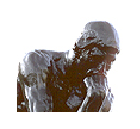
\epsfig{file=think.eps, width=\linewidth}
    \end{minipage} &
    \begin{minipage}{0.8\linewidth}

      So I suppose you are one of 150 people working on that!

    \end{minipage} \\
    & \vspace{0cm} \\
    \begin{minipage}{0.1\linewidth}
      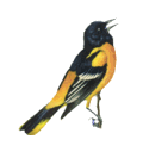
\epsfig{file=squawk.eps, width=\linewidth} \vspace{5cm}
    \end{minipage} &
    \begin{minipage}{0.8\linewidth}

      No, this is our group:
      \begin{itemize}

	\item Me

	\item Ritchie Patterson (my advisor)

	\item Karl Berkelman (theoretical calculations)

	\item Istvan Danko (actually working on a related measurement)

	\gray

	\item Rich Galik (involved in the planning stage)

	\item Dan Hennessy (involved during the data-taking stage)

      \end{itemize}

    \end{minipage} \\
  \end{tabular}
\end{center}

\begin{enumerate}

  \item Those of us who were interested formed a small working group
  to discuss how the data-taking would be conducted.  I made Toy Monte
  Carlos.

  \item We gave the data-taking procedure to \cesr, since they control
  the energy of the beams.  I stayed up all night watching the data
  come in.

  \item The data was processed (hits $\to$ tracks) by the Pass2
  committee, since this is a major computational challenge (large
  volume).  I studied systematic errors.

  \item \ldots I'm still studying systematic errors.

\end{enumerate}

\end{minipage}
\end{slide*}

% %%%%%%%%%%%%%%%%%%%%%%%%%%%%%%%%%%%%%%%%%%%%%%%%%%%%%%%%%%%%%%%%%%%%%%%%%%%

\begin{slide*}
\slideframe{}
\slideframe*[\dkblue]{Oval}
\begin{minipage}[t]{\linewidth}
\Large \black

{\huge A Systematic Error: Beam-Gas Collisions}

\vspace{0.25cm}

We want to measure the process where $e^+$ and $e^-$ actually collide,
but sometimes this happens:

\vspace{0.25cm}

\begin{center}
  \epsfig{file=beamgas.eps, width=\linewidth}
\end{center}

\vspace{0.5cm}

How do we remove these from our sample?

\vspace{0.5cm}

\begin{center}
  \begin{tabular}{p{0.29\linewidth} | p{0.31\linewidth} | p{0.3\linewidth} }
    What to do & Why this might work & Why it doesn't \\\hline

    Remove events with high $\left| \Sigma \vec{p} \cdot \hat{z} \right|$ &
      The gas atoms are at rest, so there is net momentum &
      Good events also have a wide $p_z$ distribution, because you
      don't see neutrinos \\

    Remove events with \mbox{$E_{\mbox{\small visible}}$ $\ll
      E_{\mbox{\small beam}}$} &
      Most particles pass undetected down the beam pipe &
      We do this, but you can't cut hard enough without losing data \\

    Find XYZ location of primary vertex &
      Good events only come from the collision point &
      Now you're on to something\ldots \\

  \end{tabular}
\end{center}

\end{minipage}
\end{slide*}

% %%%%%%%%%%%%%%%%%%%%%%%%%%%%%%%%%%%%%%%%%%%%%%%%%%%%%%%%%%%%%%%%%%%%%%%%%%%

\begin{slide*}
\slideframe{}
\slideframe*[\dkblue]{Oval}
\begin{minipage}[t]{\linewidth}
\Large \black

I developed a robust primary vertex-finding algorithm and plotted
where all the events in data come from:

\vspace{0.5cm}

\begin{center}
  \vspace{-0.25cm} \epsfig{file=cuts_illustration5.eps, width=0.9\linewidth} \vspace{-1.1cm}\\
\end{center}

\vspace{1cm}

\begin{itemize}

  \item Collision events are inside the red box

  \item Beam-gas events form a long strip along the beam

  \item Beam-wall collisions happen at 2 cm (where the beam pipe is)

  \item Cosmic rays are ``vertexed'' just about anywhere

  \item Some beam-halo particles interact in the denser parts of the
  silicon detector

\end{itemize}

\vspace{1cm}

{\huge Final Beam-Gas Handling Strategy:}

\vspace{0.5cm}

We extrapolate beam-gas level into the cut region (red box) and
subtract.

\end{minipage}
\end{slide*}

% %%%%%%%%%%%%%%%%%%%%%%%%%%%%%%%%%%%%%%%%%%%%%%%%%%%%%%%%%%%%%%%%%%%%%%%%%%%

\begin{slide*}
\slideframe{}
\slideframe*[\dkblue]{Oval}
\begin{minipage}[t]{\linewidth}

\begin{center}
  {\LARGE \black More Detector Internals seen by Particle Interactions} \\

  \vspace{0.75cm}

  \epsfig{file=xray.eps, width=\linewidth}
\end{center}

\end{minipage}
\end{slide*}

% %%%%%%%%%%%%%%%%%%%%%%%%%%%%%%%%%%%%%%%%%%%%%%%%%%%%%%%%%%%%%%%%%%%%%%%%%%%

\begin{slide*}
\slideframe{}
\slideframe*[\dkblue]{Oval}
\begin{minipage}[t]{\linewidth}
\Large \black

\begin{center}
  \begin{tabular}{l r}
    \begin{minipage}{0.1\linewidth}
      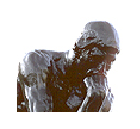
\epsfig{file=think.eps, width=\linewidth}
    \end{minipage} &
    \begin{minipage}{0.8\linewidth}

      Why are you doing this?  Are you happy with your life?

    \end{minipage} \\
    & \vspace{0cm} \\
    \begin{minipage}{0.1\linewidth}
      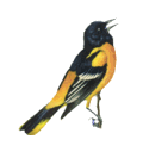
\epsfig{file=squawk.eps, width=\linewidth}
    \end{minipage} &
    \begin{minipage}{0.8\linewidth}

      I was interested in Lattice QCD, but I thought I would give
      experiment a try first.  I got hooked.

    \end{minipage} \\
  \end{tabular}

  \vspace{1cm}
\end{center}

Besides, my thesis project is a way to combine the two interests:

\vspace{0.5cm}

\begin{center}
  {\LARGE This is an experimental test of Lattice QCD}
  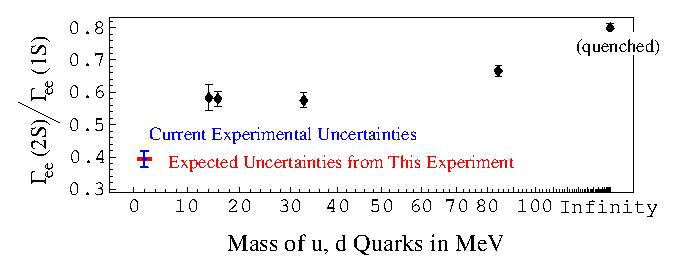
\epsfig{file=conclusion/conclusion.eps, width=\linewidth}
\end{center}

\vspace{0.5cm}

I get to interact with the theory grad student who is working on the
theoretical calculation (my anti-grad student)

\vspace{0.5cm}

\begin{center}
  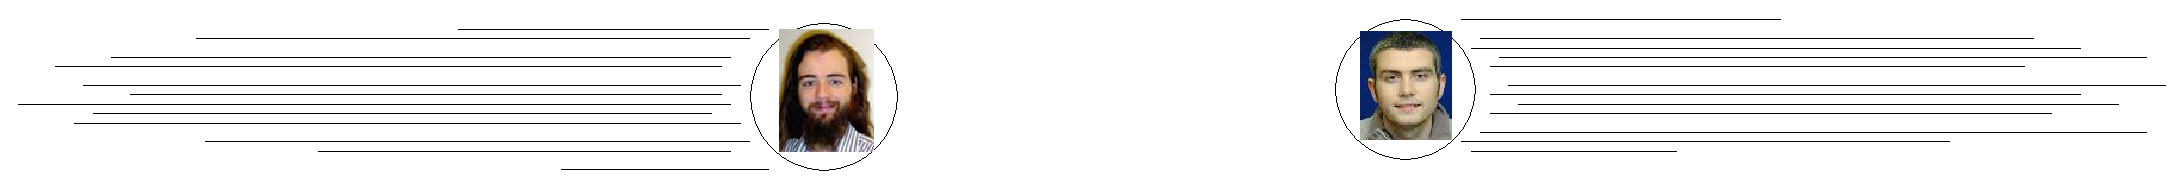
\epsfig{file=collision.eps, width=\linewidth}
\end{center}

\vspace{1cm}

And yes.

\end{minipage}
\end{slide*}

% %%%%%%%%%%%%%%%%%%%%%%%%%%%%%%%%%%%%%%%%%%%%%%%%%%%%%%%%%%%%%%%%%%%%%%%%%%%

% \begin{slide*}
% \slideframe{}
% \slideframe*[\dkblue]{Oval}
% \begin{minipage}[t]{\linewidth}
% \Large \black

% \end{minipage}
% \end{slide*}

% %%%%%%%%%%%%%%%%%%%%%%%%%%%%%%%%%%%%%%%%%%%%%%%%%%%%%%%%%%%%%%%%%%%%%%%%%%%

% \begin{slide*}
% \slideframe{}
% \slideframe*[\dkblue]{Oval}
% \begin{minipage}[t]{\linewidth}
% \Large \black

% \end{minipage}
% \end{slide*}

% %%%%%%%%%%%%%%%%%%%%%%%%%%%%%%%%%%%%%%%%%%%%%%%%%%%%%%%%%%%%%%%%%%%%%%%%%%%

% \begin{slide*}
% \slideframe{}
% \slideframe*[\dkblue]{Oval}
% \begin{minipage}[t]{\linewidth}
% \Large \black

% \end{minipage}
% \end{slide*}

% %%%%%%%%%%%%%%%%%%%%%%%%%%%%%%%%%%%%%%%%%%%%%%%%%%%%%%%%%%%%%%%%%%%%%%%%%%%

% \begin{slide*}
% \slideframe{}
% \slideframe*[\dkblue]{Oval}
% \begin{minipage}[t]{\linewidth}
% \Large \black

% \end{minipage}
% \end{slide*}

% %%%%%%%%%%%%%%%%%%%%%%%%%%%%%%%%%%%%%%%%%%%%%%%%%%%%%%%%%%%%%%%%%%%%%%%%%%%

% \begin{slide*}
% \slideframe{}
% \slideframe*[\dkblue]{Oval}
% \begin{minipage}[t]{\linewidth}
% \Large \black

% \end{minipage}
% \end{slide*}

% %%%%%%%%%%%%%%%%%%%%%%%%%%%%%%%%%%%%%%%%%%%%%%%%%%%%%%%%%%%%%%%%%%%%%%%%%%%

% \begin{slide*}
% \slideframe{}
% \slideframe*[\dkblue]{Oval}
% \begin{minipage}[t]{\linewidth}
% \Large \black

% \end{minipage}
% \end{slide*}

% %%%%%%%%%%%%%%%%%%%%%%%%%%%%%%%%%%%%%%%%%%%%%%%%%%%%%%%%%%%%%%%%%%%%%%%%%%%

% \begin{slide*}
% \slideframe{}
% \slideframe*[\dkblue]{Oval}
% \begin{minipage}[t]{\linewidth}
% \Large \black

% \end{minipage}
% \end{slide*}

% %%%%%%%%%%%%%%%%%%%%%%%%%%%%%%%%%%%%%%%%%%%%%%%%%%%%%%%%%%%%%%%%%%%%%%%%%%%

% \begin{slide*}
% \slideframe{}
% \slideframe*[\dkblue]{Oval}
% \begin{minipage}[t]{\linewidth}
% \Large \black

% \end{minipage}
% \end{slide*}

% %%%%%%%%%%%%%%%%%%%%%%%%%%%%%%%%%%%%%%%%%%%%%%%%%%%%%%%%%%%%%%%%%%%%%%%%%%%

% \begin{slide*}
% \slideframe{}
% \slideframe*[\dkblue]{Oval}
% \begin{minipage}[t]{\linewidth}
% \Large \black

% \end{minipage}
% \end{slide*}

% %%%%%%%%%%%%%%%%%%%%%%%%%%%%%%%%%%%%%%%%%%%%%%%%%%%%%%%%%%%%%%%%%%%%%%%%%%%

% \begin{slide*}
% \slideframe{}
% \slideframe*[\dkblue]{Oval}
% \begin{minipage}[t]{\linewidth}
% \Large \black

% \end{minipage}
% \end{slide*}

% %%%%%%%%%%%%%%%%%%%%%%%%%%%%%%%%%%%%%%%%%%%%%%%%%%%%%%%%%%%%%%%%%%%%%%%%%%%

% \begin{slide*}
% \slideframe{}
% \slideframe*[\dkblue]{Oval}
% \begin{minipage}[t]{\linewidth}
% \Large \black

% \end{minipage}
% \end{slide*}

% %%%%%%%%%%%%%%%%%%%%%%%%%%%%%%%%%%%%%%%%%%%%%%%%%%%%%%%%%%%%%%%%%%%%%%%%%%%

% \begin{slide*}
% \slideframe{}
% \slideframe*[\dkblue]{Oval}
% \begin{minipage}[t]{\linewidth}
% \Large \black

% \end{minipage}
% \end{slide*}

% %%%%%%%%%%%%%%%%%%%%%%%%%%%%%%%%%%%%%%%%%%%%%%%%%%%%%%%%%%%%%%%%%%%%%%%%%%%

% \begin{slide*}
% \slideframe{}
% \slideframe*[\dkblue]{Oval}
% \begin{minipage}[t]{\linewidth}
% \Large \black

% \end{minipage}
% \end{slide*}

% %%%%%%%%%%%%%%%%%%%%%%%%%%%%%%%%%%%%%%%%%%%%%%%%%%%%%%%%%%%%%%%%%%%%%%%%%%%

% \begin{slide*}
% \slideframe{}
% \slideframe*[\dkblue]{Oval}
% \begin{minipage}[t]{\linewidth}
% \Large \black

% \end{minipage}
% \end{slide*}

\end{document}

